\documentclass{article}

\usepackage{hyperref}                 % Hyperlinks
\hypersetup{
	hidelinks,                        % Hide link boxes
	colorlinks = true,
	citecolor = cyan,
	urlcolor = black,
	linkcolor = magenta,
	pdftitle = {Thresholds Without Error Bars: A Statistical Audit of Frontier AI Safety Evaluations},
	pdfauthor = {Tom Kimpson},
	pdfsubject = {Statistical audit of AI safety evaluations},
	pdfkeywords = {AI safety, dangerous-capability evaluations, statistical power, frontier safety frameworks, confidence intervals}
}
\usepackage{arxiv}
\usepackage{amsmath}
\usepackage[utf8]{inputenc} % allow utf-8 input
\usepackage[T1]{fontenc}    % use 8-bit T1 fonts
\usepackage{url}            % simple URL typesetting
\usepackage{booktabs}       % professional-quality tables
\usepackage{amsfonts}       % blackboard math symbols
\usepackage{amssymb}        % math symbols
\usepackage{nicefrac}       % compact symbols for 1/2, etc.
\usepackage{microtype}      % microtypography
\usepackage{cleveref}       % smart cross-referencing
\usepackage{graphicx}
\graphicspath{{figures/}}
\usepackage{natbib}
\usepackage{doi}
\usepackage[table]{xcolor}   % [table] loads colortbl for \rowcolor (census highlight)
\definecolor{auditrow}{rgb}{0.90,0.94,1.0}  % shading for the audited census rows
\usepackage{subcaption}
% Captions sit below our tables (arxiv.sty assumes above and zeroes the gap there),
% so restore a 7pt gap between the tabular and the caption.
\captionsetup[table]{position=below,skip=7pt}
\usepackage{longtable}       % multi-page census table (appendix)
\usepackage{pdflscape}       % rotate the wide census table to landscape (appendix)

% Exact census counts, generated by scripts/make_tables.py.
% GENERATED by scripts/make_tables.py -- exact census counts.
\newcommand{\CensusTotal}{98}
\newcommand{\CensusWithN}{83}
\newcommand{\CensusNoN}{15}
\newcommand{\CensusUncertainty}{15}
\newcommand{\CensusInterval}{9}
\newcommand{\CensusBarePm}{6}
\newcommand{\CensusPostRows}{31}


\title{Thresholds Without Error Bars: A Statistical Audit of Frontier AI Safety Evaluations}

\renewcommand{\shorttitle}{Thresholds without error bars}


% Here you can change the date presented in the paper title
%\date{September 9, 1985}
% Or remove it
%\date{}


% Multiple affiliations variant of author block
\usepackage{authblk}
\renewcommand\Authfont{\bfseries}
\setlength{\affilsep}{0em}
\author[1]{Tom Kimpson}
% Add co-authors as needed:
%\author[1]{Co-Author Name}
\affil[1]{School of Mathematics and Statistics, The University of Melbourne, Parkville, VIC 3010, Australia\\
Correspondence: \texttt{tom.kimpson@unimelb.edu.au}}
%\affil[2]{Department, Institution, City, Country}



% Suppress the `A preprint' label under the title and in the running header
\renewcommand{\headeright}{}
\renewcommand{\undertitle}{}


\begin{document}
\maketitle


\begin{abstract}

Frontier AI governance often compares dangerous-capability scores with declared
thresholds. A deterministic rule on one fixed benchmark needs no sampling inference; but
when the score is used as evidence about reruns, new tasks, latent capability, or deployment
performance, external audit requires a stated estimand, quantified uncertainty, and a
decision rule. We assemble a structured corpus of \CensusTotal{} eligible, source-reported
evaluation records from 26 public documents. \CensusNoUncertainty{} records report no
uncertainty, \CensusBarePm{} give only an unlabelled ``$\pm$'' dispersion, and
\CensusInterval{} give a proper interval. We then analyse ten model-level threshold
comparisons under explicit IID-Bernoulli working models. With a deployment-aligned one-sided
95\% Wilson rule, two of six direct-count results are unresolved. For four SWE-bench results,
two are unresolved when tasks are the sampling unit and one when task-runs are; the public
aggregates do not identify which variance model should govern. As a separate case study,
all nine allowed arm-size combinations and all three conventional readings considered for
the Opus~4 bio-uplift trial's unlabelled dispersion retain its $2.53\times$ estimate across
the $2.8\times$ supplementary acceptable-risk line. These conditional reconstructions do
not adjudicate the developers' decisions. They show that the published record often lacks
the information needed to verify how evidence maps to action. We recommend reporting the
estimand, uncertainty interval, and decision rule for every thresholded result.
\end{abstract}


\keywords{AI safety \and dangerous-capability evaluations \and statistical power \and frontier safety frameworks \and confidence intervals}



\section{Introduction}

The increasing capabilities of frontier AI models have led many labs to publish safety frameworks. Some examples include Anthropic's Responsible Scaling
Policy (RSP) \citep{anthropic2026rsp}, OpenAI's Preparedness Framework
\citep{openai2025preparedness}, and Google DeepMind's Frontier Safety Framework
\citep{deepmind2025fsf}. These frameworks evaluate the dangerous capabilities of a model to decide whether it is safe to deploy. The standard procedure is as follows: an evaluation produces a score, the score is compared against a declared threshold, and the comparison between score and threshold decides whether a model is in some dangerous regime. For example, an evaluation might measure the uplift in a user's ability to cause harm with and without using AI (say in some biosafety-related domain; \citealp{fmf2025biosafety}); a model is classified as safe if the uplift is less than some threshold (``the uplift was 2\% relative to a threshold of 5\% so the model is safe'').

When an evaluation score is used to infer performance beyond the observed benchmark or
trials, its statistical uncertainty matters. This conditional distinction is increasingly
recognised in work treating model evaluations as scientific experiments
\citep{miller2024adding,madaan2024quantifying,heineman2025signal,bowyer2025position,raman2025intolerable}.


However, while the importance of a statistical approach to model evaluations is clear, the extent to which published evaluations adhere to one is not. Statistical claims require a stated sample size, a stated uncertainty on the score, and a threshold that is sufficiently precise and quantitative to compare against. It is not known whether published frontier safety results currently meet those requirements, and accordingly how far the corresponding safety claims can be trusted. For example, if the statistical uncertainty on the score is large relative to the difference between the score and the threshold, the evaluation cannot meaningfully separate ``safe'' from ``dangerous''. Concretely, we are interested in the question \emph{can published model evaluations statistically distinguish ``safe'' from ``dangerous'' with the confidence that a deployment decision requires?}

Making this precise requires naming the estimand. A score--threshold comparison becomes a
statistical test only after specifying the source of randomness and target population. Our
reconstructions therefore use row-specific working estimands. For METR they concern reruns
of one fixed task under a stable configuration; for the bioweapons set they treat the
selected, manually graded questions as exchangeable items; for SWE-bench we show both
task- and task-run-level conventions. The public aggregates do not identify prompt,
scaffold, grader, or cluster variance, and they do not validate these exchangeability
assumptions. Where policy is defined directly on a fixed empirical benchmark, no sampling
uncertainty is required merely to check whether that policy rule was crossed, although
generalisation beyond the observed benchmark remains a separate question.

We address this question by auditing the published record of AI safety frameworks. We compile a structured corpus of \CensusTotal{} governance-relevant evaluation records spanning the safety frameworks of Anthropic, OpenAI, and Google DeepMind, together with results from third-party evaluators (METR, UK~AISI, Apollo). For each result we ask: is a sample size reported, is the score's
uncertainty stated, and is the threshold even quantitative? Where possible, we reconstruct the omitted uncertainty on the score and test whether the score and threshold can be statistically separated. Numerous previous works have performed reviews of AI safety frameworks. \cite{stelling2025evaluating} assess 12 frameworks against governance criteria, finding them under-specified. \cite{tong2026foresight} similarly publish an AI safety benchmark based on governance criteria. \cite{fli2025index} also publish a comprehensive AI safety index. \cite{bommasani2023fmti} evaluate the transparency of frontier models. What no prior work does is ask whether the published evaluations used in frontier safety have the statistical resolving power to support the distinction between ``safe'' and ``unsafe'' that is claimed. The closest ancestor to this work is \citet{miller2024adding}, who argues that evaluation scores should carry error bars; we build on this by first investigating which published safety evaluations actually report those error bars, and second, whether the safe-versus-dangerous conclusions drawn from them still hold once the error bars are taken into account.


This paper is organised as follows. \Cref{sec:census} presents the structured corpus. \Cref{sec:audit} gives conditional reconstructions for a model-level subset, \Cref{sec:uplift} considers the Opus~4 human bio-uplift trial, and \Cref{sec:discussion} presents implications and recommendations.



\section{Structured corpus of governance-relevant evaluations}
\label{sec:census}

We screened the 26 version-pinned public documents in
\texttt{data/raw/sources/MANIFEST.md}, current through 30 June 2026. They cover four
framework families: Anthropic system cards and its RSP; OpenAI system cards and its
Preparedness Framework; Google DeepMind's Frontier Safety Framework, evaluation paper,
and Gemini reports \citep{phuong2024evaluating,deepmind2025gemini3}; and public reports
from METR, UK~AISI, and Apollo. This is a fixed, purposive document frame, not a claim to
have enumerated every safety evaluation ever published. Fractions below describe this
corpus only.

The record unit is one source-reported table row or prose result whose score is mapped to a
safety-relevant capability or deployment determination. We retain the source's displayed
granularity rather than manufacturing unavailable disaggregates, and assign every record a
stable ID. A record can therefore contain a shared result for more than one model or metric;
model-specific results are expanded only for the audit in \Cref{sec:audit}. This unit
supports an analysis of reporting practice, not an estimate of the number of latent
evaluation outcomes. We screened \CensusScreened{} records and exclude two from the primary
corpus: T7 describes a benchmark but gives no evaluated-model result, and A32 was explicitly
not used for the RSP determination. The \CensusTotal{} eligible records and both exclusions
are listed in \Cref{tab:census}.

The canonical coding file, \texttt{data/raw/census\_records.csv}, records eligibility,
exclusion reason, denominator status, and uncertainty class explicitly. A ``score $n$'' is
a denominator tied to the displayed score; ``partial $n$'' is numerical sample information
that does not identify that denominator. A proper interval states a coverage level and
inferential construction; an unlabelled ``$\pm$'' is coded separately. These are data
fields, not text heuristics. \Cref{tab:census-sensitivity} reports the primary-versus-
screened coding sensitivity. Where the audit reconstructs an integer count, it uses
$k=\operatorname{round}(\hat p n)$ and reports the resulting $\pm1$ sensitivity.

% GENERATED by scripts/make_tables.py -- do not edit by hand.
\begin{table}[t]
    \centering
    \small
    \begin{tabular}{lrrrrrr}
        \toprule
        coding & records & score $n$ & partial $n$ & no $n$ & any uncertainty & proper interval \\
        \midrule
        Primary eligible corpus & 96 & 73 & 8 & 15 & 15 & 9 \\
        All screened records & 98 & 75 & 8 & 15 & 15 & 9 \\
        \bottomrule
    \end{tabular}
    \caption{Corpus-coding sensitivity. The primary corpus excludes T7 (a benchmark description with no evaluated-model result) and A32 (explicitly not used for the RSP determination). ``score $n$'' is a denominator tied to the displayed score; ``partial $n$'' is numerical sample information that does not identify that denominator. Including both screened-but-ineligible records changes the record count but not the number reporting uncertainty.}
    \label{tab:census-sensitivity}
\end{table}


%\paragraph{How rarely uncertainty is reported.}
Of the \CensusTotal{} eligible records, \CensusScoreN{} report a denominator tied to the displayed score, \CensusPartialN{} report only partial or indirect sample information, and \CensusNoN{} report none. Only \CensusUncertainty{} report any kind of uncertainty on the score. The majority (\CensusNoUncertainty{}/\CensusTotal{}) are point estimates: every Gemini~2.5 critical-capability-level determination and every cybersecurity capture-the-flag (CTF) ``$X/Y$'' solve entry in the corpus carries no uncertainty, and the only uncertainty OpenAI
attaches to any of its cards is the ``$\pm$'' margin on the externally run UK~AISI cyber results in the GPT-5.5 card (pass@5 $=90.5\% \pm 12.9\%$), which sits against a qualitative capability tier rather than a stated line. The omission is most severe when a small sample size coincides with a governance decision that depends on the score; with few trials the sampling error is large, but no error bar is placed on the number that informs the decision. This recurs across CTF suites of 4--13 challenges, the 33-question bioweapons knowledge set, and ARC's 12 autonomous-replication tasks. Of the \CensusUncertainty{} results that do state a dispersion, only \CensusInterval{} are proper confidence or credible intervals that make an explicit probabilistic claim about where the true value lies, with a stated coverage level and interpretation --- e.g.\ ``95\% CI [0.31, 0.52]'' or ``bootstrapped 95\% CI''. The remaining \CensusBarePm{} are unlabelled ``$\pm$'' dispersions; it is not clear whether these represent a standard deviation, a standard error, a full range, or something else, and no confidence level is named.

The \CensusInterval{} proper intervals cluster in a handful of sources: METR (bootstrapped 95\%
CIs) and DeepMind's 2024 paper (bootstrapped CIs plus one-sided credible intervals for
self-proliferation) supply seven of the \CensusInterval{} between them; a 95\% CI on Gemini~3~Pro's RE-Bench score and error bars on Opus~4.7's capability-trajectory metric provide the remaining two. However, of the \CensusInterval{}, only DeepMind's credible interval (census ID D6) is placed against a numeric go/no-go criterion that informs a decision rule --- and that row comes from DeepMind's 2024 research paper \citep{phuong2024evaluating}, not from a production Gemini card. The METR autonomy and RE-Bench CIs (T3--T6) and DeepMind's persuasion CIs (D1, D2) carry no threshold at all; the latter two are compared against a prose tier (Gemini~3~Pro, D18) and a trajectory slope (Opus~4.7, A30) rather than a threshold the interval could be tested against. A CI or error bar with no threshold beside it can still inform qualitative judgment, model comparison, or trend assessment, but it cannot inform the point-versus-threshold decision it would supposedly support. Thus even the few interval-reporting records rarely connect that interval to an operative quantitative decision rule; most other classifications in the corpus report point estimates only.



A number of the thresholds in the corpus are not numeric go/no-go lines, but instead qualitative classifications. For example, OpenAI's Preparedness Framework issues its determinations as Low / Medium / High /
Critical tiers (numeric lines appear in its cards, but are recorded as indicative rather than operative; \Cref{sec:audit}); DeepMind's deployed Frontier Safety Framework names critical capability levels
qualitatively (the numeric criterion of D6 appears only in its 2024 research paper); Anthropic states that it has no formal cyber threshold
at any ASL level (the RSP does state numeric lines for the bioweapons-knowledge and autonomy evaluations, the rows that survive to the audit of \Cref{sec:audit}). These qualitative thresholds still sit against a quantitative evaluation score that carries
no uncertainty. As a result, the governance decision rests on two layers of judgment: the
noisy, unquantified evaluation score, and an undisclosed mapping from that score to a
qualitative tier. The second mapping may be reasonable, but it is typically unpublished, so
no external party can check it. A qualitative threshold does not remove the underlying
sampling noise. Instead it leaves that noise unquantified, adds a second uninspectable layer on
top, and removes any external object against which to test the decision.

\section{Bernoulli audit: can each pass rate resolve its own threshold?}
\label{sec:audit}

%Which rows are auditable
The corpus, \Cref{tab:census}, records evaluation results published by several AI safety frameworks. We now ask a more specific, conditional question. Given a score compared with a numerical threshold, can a stated working model resolve the score from that threshold using the public aggregates? Specifically, in this section we consider a record reconstructable if an evaluation is represented as an integer pass count $k$ over $n$ Bernoulli trials
(reported, or reconstructed as in \Cref{sec:census}) and compared against a
numeric threshold $\tau$ defined on that same proportion. Additionally, the record must use this $\{k, n, \tau\}$ tuple to make a decision. Across the frameworks in the corpus, only a small minority of results satisfy these two conditions. For example, in its production cards, DeepMind reports clean integer counts (Gemini~3~Pro solves 11 of 12 hard cyber
challenges, 0 of 13 end-to-end, 3 of 11 situational-awareness tasks) but maps them to qualitative capability levels.\footnote{The one DeepMind row with a numeric criterion (D6) sits in its 2024 research paper, not a card, and reports a modelled success probability, not a pass count.} OpenAI does provide quantitative thresholds and sample sizes, but its published scores are typically transforms (e.g.\ a Spearman correlation, a refusal-adjusted rate) that do not let us recover $k$; when $k$ is recoverable, $\tau$ is only indicative and the verdict is qualitative, so there is no operative threshold to test $k$ against. Anthropic provides both pass counts and operative thresholds $\tau$. \Cref{tab:anatomy} summarises the auditability of different developers.

\begin{table}[t]
    \centering
    \scriptsize
    \resizebox{\textwidth}{!}{%
    \begin{tabular}{lllllll}
        \toprule
        developer / card & threshold $\tau$ & $n$ & count $k$ recoverable? & uncertainty & decision rule & auditable? \\
        \midrule
        DeepMind Gemini~3~Pro (cyber, misalign.\ tasks) & no (prose CCL) & yes (12, 13, 11, 4) & \textbf{yes} (11, 0, 3, 1) & no & prose CCL / alert & no \\
        OpenAI GPT-5.5 (bio pass@$k$) & yes (indicative) & yes (156; 43/492; 550) & partial (pass@1 yes; reward@4 no) & partial (UK~AISI $\pm$) & prose High tier & no \\
        OpenAI GPT-5.6 Prev.\ (bio evals) & yes (indicative) & yes (350, 108, 60, 156) & partial (\% yes; Spearman no) & no & prose High tier & no \\
        Anthropic Opus~4/4.5 (bioweap.\ 33; SWE-b.\ 45) & \textbf{yes} (RSP) & yes (33; 45) & \textbf{yes} (17/33; 21/45) & no & RSP threshold & \textbf{yes} \\
        Anthropic Opus~4.6--4.8 (SWE-b.; AECI traj.) & yes (RSP) & partial & no (run-mean, not task count) & no & prose / trajectory & no \\
        \bottomrule
    \end{tabular}%
    }
    \caption{Representative examples of the auditability of published evaluation
    results. We present a selection of cards from each developer. A result is auditable only if it pairs an
    operative numeric threshold $\tau$ with a recoverable pass count $k$ out of $n$
    trials (reported or reconstructed) on the same
    evaluation, ideally with an uncertainty interval tied to a decision rule. Each row
    describes only the evaluations named in its label, not every evaluation in that card.}
    \label{tab:anatomy}
\end{table}

%Overview/explanation of table 2
Only a small model-level subset is reconstructable. Ten results pair a reported or
reconstructed count $\{k,n\}$ with an operative numeric threshold $\tau$, all from
Anthropic cards. The source record A4 gives the same 17/33 result for Opus~4 and Sonnet~4;
because this audit's unit is capability $\times$ model, both appear separately in
\Cref{tab:audit}. This makes the model-level denominator explicit without pretending that
the shared source record contains independent data.

We analyse all ten under an IID Bernoulli \emph{working model}, not as an observed property
of the designs. For the three METR results, this treats 29--46 stochastic reruns of one
fixed data-deduplication task as independent and identically configured. For the three
bioweapons-knowledge results, it treats the deliberately constructed, manually graded 33
questions as exchangeable draws and ignores grader variation. For the four SWE-bench
results, the published score is a ten-run mean; we show a task-generalisation convention
with $n$ equal to tasks and a run-generalisation sensitivity with
$n=\text{tasks}\times10$. The released aggregates cannot test any of these assumptions or
identify the relevant variance components.

The primary decision is directional. If $\hat p<\tau$, safety relative to the line is
resolved only when the one-sided 95\% Wilson upper bound is below $\tau$; if
$\hat p>\tau$, the corresponding lower bound must exceed $\tau$. The table displays both
one-sided 95\% endpoints (equivalently, the endpoints of a central 90\% interval), but each
decision uses only the bound in the observed direction. Equality is unresolved. A central
two-sided 95\% Wilson interval is a declared sensitivity, not the primary rule. Wilson is
used because the row sizes are small \citep{brown2001interval}; construction and confidence-
level sensitivities appear in \Cref{app:robustness}.

We also report the one-sided sample size $n_{\mathrm{req}}$ needed for 95\% power at the
observed gap, following \citet{miller2024adding}. Because the effect estimate is itself
noisy, this is an order-of-magnitude diagnostic rather than a design prescription. Under a
uniform prior the posterior is $\mathrm{Beta}(k+1,n-k+1)$, and $P(p>\tau)$ is its upper
tail. Reconstructed counts are perturbed by $\pm1$. Finally, for rows where item clustering
is meaningful, we report the design effect at which the primary verdict changes and its ICC
translation across $m\in\{5,10,20\}$. The source cards publish neither cluster labels nor
sizes. Item clustering is inapplicable to the single-task METR rows, but their reruns can
still share prompts, scaffolds, and infrastructure; independence remains a working
assumption.


% GENERATED by scripts/make_tables.py -- do not edit by hand.
\begin{table}[t]
    \centering
    \small
    \begin{tabular}{llcccccc}
        \toprule
        eval & model & $n$ & $\hat p$ & directional 95\% bounds & $\tau$ & primary class & $P(p>\tau)$ \\
        \midrule
        SWE-bench hard (A28) & Opus 4.5 & 45 & 0.47 & 0.35--0.59 & 0.50 & \textbf{indeterminate} & 0.329 \\
        SWE-bench hard (A12) & Opus 4 & 42 & 0.40 & 0.29--0.53 & 0.50 & \textbf{indeterminate} & 0.111 \\
        SWE-bench hard (A13) & Sonnet 4 & 42 & 0.36 & 0.25--0.48 & 0.50 & below demonstrated & 0.033 \\
        SWE-bench hard (A14) & Claude 3.7 & 42 & 0.24 & 0.15--0.36 & 0.50 & below demonstrated & 0.000 \\
        METR dedup (A15) & Opus 4 & 46 & 0.33 & 0.22--0.45 & 0.20 & above demonstrated & 0.983 \\
        METR dedup (A16) & Sonnet 4 & 29 & 0.28 & 0.16--0.43 & 0.20 & \textbf{indeterminate} & 0.871 \\
        METR dedup (A17) & Claude 3.7 & 30 & 0.13 & 0.06--0.27 & 0.20 & \textbf{indeterminate} & 0.229 \\
        Bioweapons knowl. (A4) & Opus 4 & 33 & 0.52 & 0.38--0.65 & 0.82 & below demonstrated & 0.000 \\
        Bioweapons knowl. (A4) & Sonnet 4 & 33 & 0.52 & 0.38--0.65 & 0.82 & below demonstrated & 0.000 \\
        Bioweapons knowl. (A5) & Claude 3.7 & 33 & 0.52 & 0.38--0.65 & 0.82 & below demonstrated & 0.000 \\
        \bottomrule
    \end{tabular}
    \caption{Conditional IID-Bernoulli audit of ten model-level results. The
    primary class is three-way: ``below demonstrated'' when the one-sided 95\%
    upper Wilson bound is below $\tau$, ``above demonstrated'' when the
    one-sided 95\% lower bound is above $\tau$, and ``indeterminate'' otherwise.
    These are two separate claims, each controlled at $\alpha=0.05$; the displayed
    pair equals the endpoints of a central 90\% interval and is \emph{not} a
    simultaneous 95\% classification. Below/indeterminate/above counts are
    3/2/1 for the six direct-count rows, 2/2/0 for
    SWE-bench at task level, and 3/1/0 under the run-level
    sensitivity ($n=\text{tasks}\times10$).
    $P(p>\tau)$ is the Beta posterior probability under a uniform prior.
    The code after each eval name (e.g.\ ``(A5)'') is that row's ID in the full
    census, \Cref{tab:census}, where these rows are shaded. Full two-sided,
    sample-size, count, and clustering sensitivities appear in
    \Cref{tab:audit-sensitivity}.}
    \label{tab:audit}
\end{table}




%Results, including into of figure 1
\Cref{fig:straddle} plots the primary directional bounds. Among the six direct-count
results, two are unresolved: the Sonnet~4 and Claude~3.7 METR rerun results. Among the four
SWE-bench results, the task-level working model leaves Opus~4.5 and Opus~4 unresolved
(two of four); the run-level sensitivity leaves only Opus~4.5 unresolved (one of four).
These tiers are more informative than one pooled fraction because they expose the sampling-
unit dependence. The central two-sided 95\% sensitivity leaves five of ten unresolved under
task-level SWE denominators and three of ten when the SWE rows use run-level denominators.
For scale, A28 (Opus~4.5 SWE-bench hard) has
$n_{\mathrm{req}}\approx2430$ tasks under the stated one-sided approximation, compared with
45 observed tasks.



The unresolved rows occur on both sides of a threshold. When a score below a concern line
has an upper bound reaching the line, it does not demonstrate below-threshold performance.
When a score above a line has a lower bound reaching below it, it does not demonstrate that
the line was crossed. The governance consequence depends on the stated loss function and
decision rule; statistical non-resolution alone does not say which action was wrong.


The grey bars show the illustrative ICC$=0.2$ sensitivity at the reference cluster size.
A positive design effect can make a resolved row unresolved, never the reverse. The last
table column avoids treating one chosen $m$ as a fact: it translates each critical design
effect at $m=5,10,20$. For the bioweapons rows, for example, the primary critical DEFF is
7.52; it is impossible at $m=5$ but corresponds to possible ICCs of 0.724 and 0.343 at
$m=10$ and $m=20$. With unpublished clusters, no claim of immunity to ``any possible
clustering'' is warranted.



\begin{figure}[t]
    \centering
    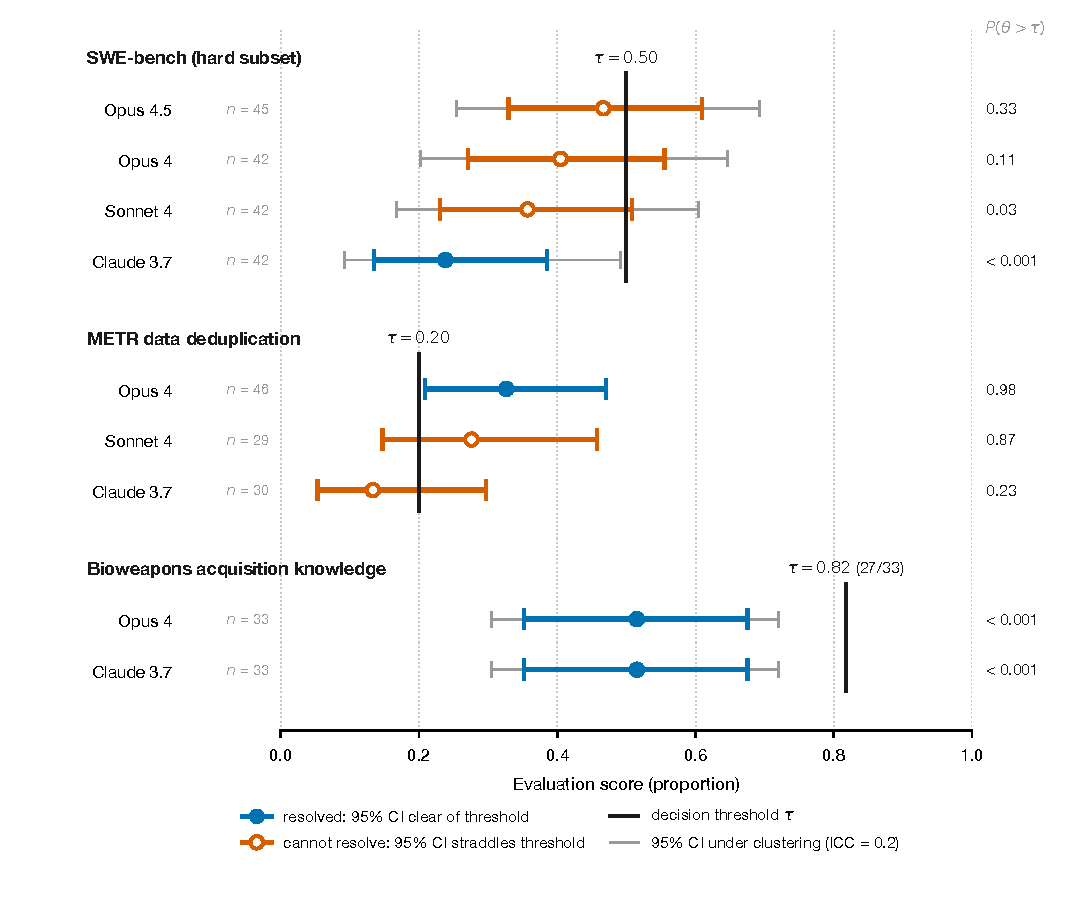
\includegraphics[width=\linewidth]{ci_straddle.pdf}
    \caption{Primary one-sided 95\% Wilson directional bounds for the ten model-level
    results under the stated IID working models. Each row shows the reported score (point) and its bounds
    (thick bar) against the decision threshold $\tau$ for its evaluation family (black
    vertical line). Open orange markers mark intervals that cross the threshold;
    these rows cannot be placed on the observed side of the line at the one-sided 95\% level. Filled
    blue markers mark intervals that lie entirely on one side; these rows resolve the
    comparison. Thin grey whiskers show each interval recomputed at the effective sample
    size under item clustering ($\mathrm{ICC}=0.2$ at the assumed cluster size,
    \Cref{sec:audit}). The METR rows are repeated trials of one task, so item clustering does not
    apply, although common-condition dependence can remain. The right-hand column gives the Beta posterior probability
    $P(p>\tau)$ that the true pass rate $p$ exceeds the threshold (\Cref{sec:audit}).}
    \label{fig:straddle}
\end{figure}




\section{Case study: bio-uplift trial}
\label{sec:uplift}

The Opus~4 human bio-uplift trial (A1) reports a ratio of continuous-rubric arm
means and therefore falls outside \Cref{sec:audit}. Each arm contained 8--10 participants,
but the card does not give the arm-specific counts. Third-party graders scored participants'
bioweapon acquisition plans. The published control and Opus~4 means are
$25\%\pm13\%$ and $63\%\pm13\%$, giving $2.53\times$ from the unrounded means. The same
card section uses $2.8\times$ and $5\times$ as supplementary threat-analysis heuristics;
they are not binding RSP thresholds.

We use Fieller's theorem \citep{fieller1954} for the ratio of two independent means. The
per-participant data and the meaning of ``$\pm13\%$'' are unavailable, so we evaluate three
conventional readings: participant SD, arm-mean SE, and 95\%-CI half-width. For the SD
reading, we enumerate every ordered $(n_C,n_T)\in\{8,9,10\}^2$ pair and use the
Welch--Satterthwaite degrees of freedom derived from the two arm-mean variances. All nine
sets contain $2.8\times$; their endpoints range from $1.73\times$ to $4.24\times$.
The CI-half-width reading gives $1.56\times$--$5.35\times$. Under the SE reading, the
unconstrained Fieller set is disconnected,
$(-\infty,-131.18]\cup[1.05,\infty)$. Because the target arm means and their ratio are
nonnegative, intersecting with that stated parameter space yields the displayed
$[1.05,\infty)$ ray. Collapsing the real-line set without this restriction would be
incorrect. Thus every reading considered retains $2.8\times$; under the equal-arm SD
illustration, the upper bound first falls below that line at about 119 participants per arm.

Anthropic did not read the $2.53\times$ as below the line; it concluded the result was ``sufficiently close that we are unable to rule out ASL-3'' and escalated. ``Sufficiently close'' is itself a claim about uncertainty: it concedes that the trial cannot place the score on one side of the threshold, which is what our reconstructed intervals show. It is possible that Anthropic computed such intervals internally and escalated on that basis. The card does not say. It publishes only a bare point estimate against a numeric line, so an outside reader cannot tell whether the escalation rests on a quantified analysis or on an unaided judgment call, and has no way to check where the same judgment would place the next model. The thresholds were never binding policy: the RSP's CBRN thresholds are qualitative, and the $2.8\times$/$5\times$ figures appear in the card only as supplementary working. But readers take a published number at face value, as a precise figure carrying no uncertainty, whatever its formal standing.

% GENERATED by scripts/make_tables.py -- do not edit by hand.
\begin{table}[t]
    \centering
    \small
    \begin{tabular}{llllll}
        \toprule
        reading of ``$\pm 13\%$'' & arm & Fieller 95\% set & delta 95\% CI & bootstrap 95\% CI & verdict \\
        \midrule
        SD & 8 & 1.7$\times$--4.5$\times$ & 1.7$\times$--3.7$\times$ & 1.8$\times$--3.9$\times$ & straddles $2.8\times$ \\
        SD & 9 & 1.7$\times$--4.3$\times$ & 1.8$\times$--3.6$\times$ & 1.8$\times$--3.8$\times$ & straddles $2.8\times$ \\
        SD & 10 & 1.8$\times$--4.1$\times$ & 1.8$\times$--3.6$\times$ & 1.8$\times$--3.7$\times$ & straddles $2.8\times$ \\
        SE & $n$-free & 1.1$\times$--$\infty$\,(unbounded) & 0.8$\times$--7.5$\times$ & 1.0$\times$--46.0$\times$ & straddles $2.8\times$; reaches $5\times$ \\
        CI half-width & $n$-free & 1.6$\times$--5.3$\times$ & 1.4$\times$--4.4$\times$ & 1.5$\times$--4.9$\times$ & straddles $2.8\times$; reaches $5\times$ \\
        \bottomrule
    \end{tabular}
    \caption{Uplift-ratio interval for the Opus~4 bio-uplift trial
    ($0.63/0.25 = 2.52\times$; the card reports $2.53\times$ from unrounded means),
    computed as a ratio of two arm means propagating the card's unlabelled
    ``$\pm 13\%$'' dispersion under every admissible reading. Fieller (headline)
    inverts the exact test, at the small-sample $t(\mathrm{df}=n-1)$ critical value
    where a per-arm $n$ is defined (the SD reading) and at the normal $z$ for the
    $n$-free readings; the delta method is a linearisation check that stays finite
    even when the exact set is unbounded; the parametric bootstrap draws
    scaled-Beta arms on $[0,100]$. \textbf{Every reading straddles the
    $2.8\times$ acceptable line}; under the most conventional (SD) reading the set
    is bounded and also excludes the $5\times$ significant-risk line. Endpoints are
    given to one decimal because propagating the card's integer-rounded inputs
    shifts each by $0.1$--$0.4\times$, so only the binary straddle verdict is
    rounding-robust. Under the standard-error reading the control mean sits just
    below significance at 95\% ($25/13 \approx 1.92 < 1.96$), so the Fieller set is
    then \emph{unbounded above} and the finite delta interval is a linearisation
    artifact; this prong is conditional on that reading and on the inputs' rounding
    (a control mean of $25.5$ or a dispersion of $12.7$ would bound it), whereas the
    straddle holds at every corner.}
    \label{tab:uplift}
\end{table}



\begin{figure}[t]
    \centering
    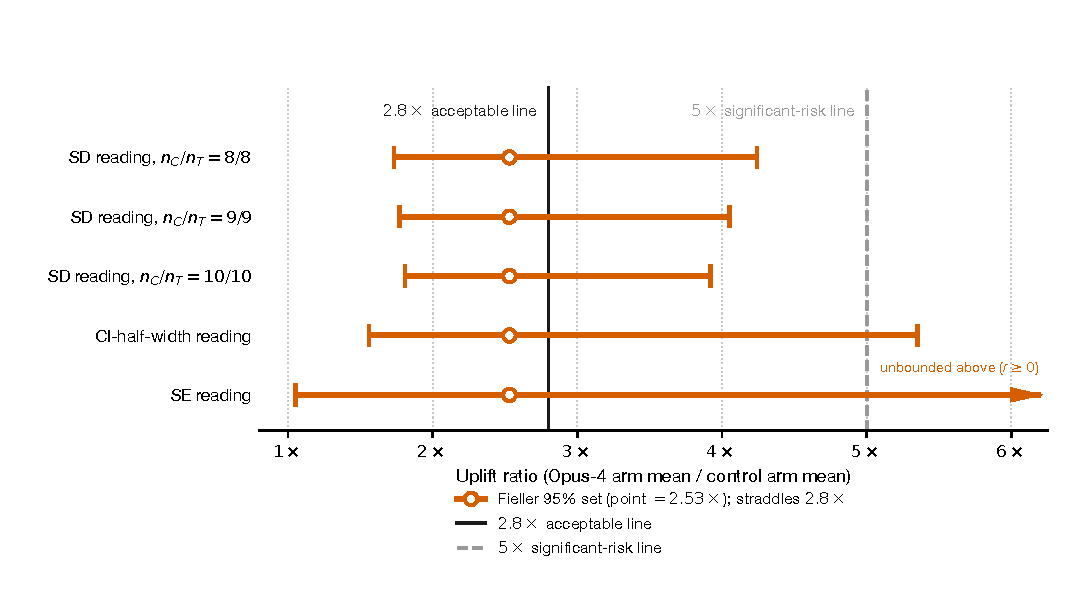
\includegraphics[width=0.92\linewidth]{uplift_straddle.pdf}
    \caption{Fieller 95\% confidence sets for the Opus~4 bio-uplift ratio, computed under
    each of the three conventional readings we consider for the card's unlabelled ``$\pm 13\%$'' dispersion. Each row
    shows the reported $2.53\times$ estimate (open marker) and its confidence set against
    the $2.8\times$ acceptable line (black) and the $5\times$ significant-risk line (grey
    dashed). The standard-deviation reading (Welch $t$, shown at equal-arm $n=8,9,10$; all
    unequal combinations appear in \Cref{tab:uplift}) gives bounded intervals within
    $1.73\times$--$4.24\times$, which exclude $5\times$. The
    CI-half-width reading reaches $5\times$. The standard-error reading is unbounded
    above after restriction to nonnegative ratios; its unconstrained real-line set is
    disjoint (\Cref{sec:uplift}). The card reports arm means only to the nearest percent, so
    the exact interval endpoints shift slightly with that rounding; the finding that every
    interval straddles the $2.8\times$ line does not.}
    \label{fig:uplift}
\end{figure}



\section{Discussion}
\label{sec:discussion}

% ¶1 — the frame: point-vs-threshold is an implicit hypothesis test, run without uncertainty
AI safety frameworks frequently compare point estimates with quantitative thresholds. A
framework may validly define a deterministic policy rule on the observed benchmark. The
statistical issue begins when that observation is offered as evidence about reruns, new
tasks, latent capability, or deployment performance. For those generalisations, ``below the
line'' requires an estimand and an uncertainty model; the benchmark rule alone supplies
neither.

% ¶2 — the results: the record cannot support that test
Our results concern external auditability of that inferential step, not the merits of the
underlying evidence. Only \CensusUncertainty{} of the \CensusTotal{} eligible corpus
records state any dispersion, and only \CensusInterval{} a proper interval
(\Cref{sec:census}). Ten model-level threshold comparisons and the uplift trial permit
conditional reconstructions from public aggregates. Their conclusions depend visibly on
the stated observation model: the direct-count and SWE tiers should not be compressed into
one unconditional headline.

% ¶3 — the consequence: two unlicensed claims (consumer's / producer's risk)
An unstated uncertainty does not stop anyone reading the point comparison. Instead, it leaves that reading unpoliced. A developer can report a model below a concern line the statistical evidence cannot place it below (false accept), and a critic can report a threshold as crossed that the evidence cannot place it above (false reject). Of the two, the developer's is the stronger claim, though it might appear the weaker one. ``Below the line'' reads as a null result (i.e. no danger found) but it is actually an affirmative claim that the true capability lies in the acceptable region. Establishing such a claim is a one-sided test against an upper limit, of the kind used to demonstrate non-inferiority or superiority in the statistical literature \citep{lakens2017,wellek2010}. Here the burden of proof reverses relative to a conventional test: the null hypothesis is danger ($H_0\!: p \geq \tau$), and safety must be demonstrated against it rather than assumed. A point estimate below the threshold does not meet that burden while its
interval still crosses the line: absence of evidence for danger is not evidence of safety.






% ¶4 — the governance pivot: the decisions are precautionary; the frame is the problem
None of this says the governance decisions were wrong. In the bio-uplift trial
(\Cref{sec:uplift}) Anthropic took the precautionary decision to deploy safeguards unless
danger can be ruled out. This is a decision-theoretic rule
\citep{wald1950statistical,taleb2014precautionary}. Its logic is to choose the action that
limits loss under uncertainty, rather than to test which side of the line the score falls on.
Under such a rule a straddling interval is not a defect but the very input that should
trigger caution. The principle already exists in governance
guidance: further evaluation is recommended when an interval overlaps an
intolerable-risk threshold \citep{raman2025intolerable}. However, the published
determinations cannot operationalise that guidance: an interval-overlap rule needs an
interval, and only \CensusUncertainty{} of \CensusTotal{} results report any dispersion
at all. The decisions are thus made in one frame (precautionary, uncertainty-aware)
and published in another: a point against a numeric line. Because the rule connecting
the evidence to the decision is never published, an outside party cannot verify that a
determination follows from its evidence, nor that the same rule is applied consistently
across models and developers; a calibrated escalation and an unaided judgment call leave
the same trace in the record. The statistical object the
precautionary frame calls for is already in hand: the decision-theoretic reading is
carried by the exceedance probabilities $P(p > \tau)$ reported alongside our verdicts
(\Cref{tab:audit}); had the frameworks published risk tolerances on that object, we would
have audited against those instead.

% ¶5 — the remedy: a metrology for AI safety (single, full entrance of the conformity frame)
This problem is not unique to AI safety. From the perspective of metrology, comparing a
measured value against a specification limit to issue a pass/fail statement is a \emph{conformity statement}. Such a statement is meaningless unless it carries a stated \emph{decision rule} --- a declaration, made
in advance, of how the measurement uncertainty enters the accept/reject call. Outside AI, such statements are governed by international standards that require a stated decision rule and guard band \citep{jcgm106_2012,iso14253_1}, and an accreditation regime makes stating the decision rule mandatory: every accredited testing laboratory must document its decision rule when it states conformity \citep{iso17025_2017,ilac_g8_2019}. The institutional half of an equivalent regime for AI has already been proposed: governance proposals call for the training, standardisation, and accreditation of third-party AI auditors \citep{raji2022outsider}, and a recent multi-institution framework sets out tiered assurance levels for audits of frontier developers \citep{brundage2026frontieraudit}. What is still missing is the metrological half --- an ISO/IEC~17025 analogue under which an accredited evaluator issuing ``below the line'' would be required to state its decision rule and uncertainty budget, as any calibration laboratory must: a metrology for AI safety.



%reccomendations
We make a series of recommendations that are cheap to implement. None are particularly novel; \citet{miller2024adding} already recommends reporting the sample size and the standard error beside each score. What follows restates his recommendations for the governance setting. Report sample sizes and confidence intervals for every gating evaluation. Label
uncertainty statements unambiguously as SD, SE, or CI (cf.\ the unlabelled ``$\pm 13\%$'' of \Cref{sec:uplift}). Where a threshold is quantitative, state the resolving power: the
interval on the score, or the sample size needed to resolve the declared gap. Where
clustering is plausible, report per-cluster counts so a design effect can be estimated
rather than assumed. These are best adopted as a common industry standard rather than
unilaterally: a method like ours can only scrutinise a developer that already publishes
$\tau$, $n$, and $k$, so the least transparent labs escape entirely while the most
transparent absorb the scrutiny. None of this
is beyond reach. Newer cards already report more of it (GPT-5.5 publishes sample sizes and
cyber margins; Anthropic's RSP has been revised repeatedly
\citep{openai2026gpt55,anthropic2026rsp}), and the 157-participant RAND uplift trial
\citep{rand2026uplift} shows adequately powered studies are feasible in practice. Resolving power must then be maintained rather than established once: new cyber-range and alignment benchmarks arrive continually \citep{liu2026agentcyberrange,souly2026alignment}, and a benchmark adequate today can saturate within a card cycle. Standardised evaluation tooling is closing the reporting gap on the infrastructure side \citep{uk_aisi_inspect}, but tooling does not by itself supply the decision rule. That is the last step the current cards still omit: tie the reported uncertainty to a stated decision rule, so that a margin becomes a governance conclusion rather than a number printed beside one.



\section{Limitations}
\label{sec:limitations}

Several limitations bound this audit. First, the 26-document sampling frame is purposive,
not exhaustive, and the record unit follows source display granularity; corpus fractions are
descriptive of these documents only. Second, extraction, recoding, and cell cross-checking
were AI-assisted. The repository includes locators, pinned sources, explicit coding fields,
and a row-level human sign-off sheet, but that sheet remains marked ``pending'' at this
draft stage. The exact corpus fractions must therefore pass the documented author sign-off
gate before submission. Third, the ten model-level audit results come from one developer and
do not support a cross-developer resolving-power comparison. Fourth, the public aggregates
do not validate the IID assumptions, identify SWE-bench variance components, reveal cluster
labels, separate grader variance, or label the uplift dispersion. We expose rather than
average over those choices. Finally, $n_{\mathrm{req}}$ is calculated at a noisy observed
effect and is a scale diagnostic, not a prospective design calculation.



\section{Conclusion}
\label{sec:conclusion}

Within the \CensusTotal{}-record eligible corpus, uncertainty reporting is uncommon:
\CensusNoUncertainty{} records give none and only \CensusInterval{} give a proper interval.
The conditional audit does not yield one design-invariant fraction. Under the primary
one-sided rule, two of six direct-count results are unresolved; the four SWE-bench results
give two unresolved at task level and one at run level. The Opus~4 uplift reconstruction
retains the supplementary $2.8\times$ line under all three conventional dispersion readings
considered and every allowed arm-size combination.

These findings do not show that the governance actions were unreasonable. They show that
published point estimates usually omit the information needed to distinguish a fixed-
benchmark policy check from an inference beyond that benchmark, or to verify how uncertainty
changes the action. The practical remedy is metrological: state the estimand and sampling
unit, report and label the uncertainty, and connect it to a predeclared decision rule.

\section*{Data and code availability}
All computation is implemented in the tested \texttt{evalaudit} package,
with the published facts held in a single data file and all modelling assumptions
(cluster sizes, priors) held separately in the analysis scripts. The full ICC$\times m$
sensitivity sweep is generated as a by-product of the main audit. The code and data that
reproduce every number, table, and figure in this paper are available at
\url{https://github.com/tomkimpson/AISafetyUncertaintyCensus}.

\textbf{Statement on AI usage:} An AI agent located documents and extracted the initial
corpus; later recoding and cell cross-checking were also AI-assisted. The construction pass
is not bit-reproducible. Archival auditability instead rests on the 26 pinned sources,
stable record IDs, page/section locators, \texttt{data/verification/cell\_audit.csv}, and
explicit coding in \texttt{data/raw/census\_records.csv}. Before submission, the author must
complete \texttt{data/verification/human\_signoff.csv}; it is intentionally pending in this
draft and no claim of completed human verification is made. The statistical pipeline is
procedurally reproducible with fixed seeds and regenerates its derived data, tables, and
figures via \texttt{make all}.

\section*{Competing interests}
The author has no lab affiliation and no financial or advisory relationship with any
developer whose cards this paper audits.

\bibliographystyle{plainnat}
\bibliography{references}





\appendix
\crefalias{section}{appendix} % \Cref{app:...} renders as "Appendix X", not "Section X"
% Appendix floats get an "A"-prefixed number (Table A1, ...) so a reference from
% the main text reads as "look in the appendix" rather than continuing the main
% sequence (which rendered tab:census as a misleading "Table 3").
\setcounter{table}{0}
\renewcommand{\thetable}{A\arabic{table}}
\setcounter{figure}{0}
\renewcommand{\thefigure}{A\arabic{figure}}
\section{Full structured corpus}
\label{app:census}
\Cref{tab:census} lists the \CensusTotal{} primary eligible records and the two screened
exclusions, parsed from the canonical structured CSV and spanning the Claude~4 / Gemini~2.5 / GPT-4.x
generation through the GPT-5.6~Preview card of June~2026; of the \CensusTotal{} rows,
\CensusPostRows{} are from the post-2025 generation (GPT-5.5, GPT-5.6~Preview,
Opus~4.5--4.8, Gemini~3--3.1). The main-text counts of \Cref{sec:census} are generated from
this table by \texttt{scripts/make\_tables.py}. Each row carries an ID (a framework letter
--- A, O, D, T --- plus a running number); shaded source records map to the ten model-level
results in \Cref{sec:audit}. A4 maps to two results because its shared 17/33 value is
reported for both Opus~4 and Sonnet~4.

\begin{landscape}
% GENERATED by scripts/make_tables.py -- do not edit by hand.
\begin{small}
\begin{longtable}{p{0.7cm}p{1.4cm}p{2.4cm}p{1.5cm}p{2.2cm}p{1.2cm}p{1.7cm}p{1.5cm}p{1.9cm}}
\caption{Primary structured corpus of source-reported dangerous-capability evaluation records, spanning the
Claude~4 / Gemini~2.5 / GPT-4.x generation through the GPT-5.6~Preview card of
June 2026, parsed from \texttt{data/raw/census\_records.csv}. ``uncert.'' reproduces
the source's uncertainty cell verbatim; most rows report none. Each row carries
an ID (framework letter + running number); \colorbox{auditrow}{shaded} rows are
audited in \Cref{sec:audit}, and their IDs appear beside the eval names
in \Cref{tab:audit}.}
\label{tab:census}\\
\toprule
ID & framework & domain & model & threshold & $n$ & score & uncert. & citation \\
\midrule
\endfirsthead
\multicolumn{9}{c}{\tablename\ \thetable\ -- continued}\\
\toprule
ID & framework & domain & model & threshold & $n$ & score & uncert. & citation \\
\midrule
\endhead
\midrule \multicolumn{9}{r}{continued on next page}\\
\endfoot
\bottomrule
\endlastfoot
  A1 & Anthropic & CBRN bio uplift trial & Opus 4 & ASL-3 $\ge$5$\times$; $\le$2.8$\times$ acceptable & 8--10/arm & 63\% (ctrl 25\%); 2.53$\times$ & $\pm$13\% & S4 \S{}7.2.4.1 pp.89-90 \\
  A2 & Anthropic & CBRN bio uplift trial & Sonnet 4 & same & 8--10/arm & 42\%; 1.70$\times$ & $\pm$11\% & S4 \S{}7.2.4.1 \\
  A3 & Anthropic & CBRN bio uplift trial & Claude 3.7 & $\ge$5$\times$ ($\le$2.8$\times$ ok) & NOT REPORTED & 27\%$\to$57\%; $\sim$2.1$\times$ & $\pm$9/$\pm$20-21\% & S3.7 \S{}7.1 pp.24-25 \\
\rowcolor{auditrow}   A4 & Anthropic & CBRN bioweapons knowledge Qs & Opus 4 / Sonnet 4 & 27/33 ($>$80\%) & 33 & 17/33 & none & S4 \S{}7.2.4.5 p.94 \\
\rowcolor{auditrow}   A5 & Anthropic & CBRN bioweapons knowledge Qs & Claude 3.7 & 27/33 & 33 & 17/33 & none & S3.7 \S{}7.1 p.27 \\
  A6 & Anthropic & CBRN long-form virology & Claude 3.7 & $<$50\% / $>$80\% & 13 subtasks & 69.7\% & none & S3.7 \S{}7.1 p.26 \\
  A7 & Anthropic & CBRN long-form virology t1/t2 & Opus 4 & $<$50\%/$>$80\% & NOT REPORTED & 0.83; 0.72 & none & S4 \S{}7.2.4.3 pp.91-92 \\
  A8 & Anthropic & CBRN long-form virology t1/t2 & Sonnet 4 & $<$50\%/$>$80\% & NOT REPORTED & 0.55; 0.635 & none & S4 \S{}7.2.4.3 \\
  A9 & Anthropic & CBRN creative biology & Opus 4 / Sonnet 4 & qual. & NOT REPORTED & 0.45 / 0.37 & $\pm$0.08 & S4 \S{}7.2.4.8 pp.97-98 \\
  A10 & Anthropic & CBRN DNA-synth screening evasion & Opus 4 / Sonnet 4 & $\ge$1 pathogen viable+evasive & 10 agents/6 criteria & none end-to-end & none & S4 \S{}7.2.4.6 pp.95-96 \\
  A11 & Anthropic & CBRN short-horizon comp-bio & Opus 4 / Sonnet 4 & per-eval bounds & 6 evals & 4/6 below rule-out & none & S4 \S{}7.2.4.9 pp.99-100 \\
\rowcolor{auditrow}   A12 & Anthropic & Autonomy SWE-bench Verified (hard) & Opus 4 & $>$50\% avg / 10 runs & 42 tasks & 16.6/42 & none & S4 \S{}7.3.1 pp.103-104 \\
\rowcolor{auditrow}   A13 & Anthropic & Autonomy SWE-bench Verified (hard) & Sonnet 4 & $>$50\% & 42 & 15.4/42 & none & S4 \S{}7.3.1 \\
\rowcolor{auditrow}   A14 & Anthropic & Autonomy SWE-bench Verified (hard) & Claude 3.7 & $>$50\% & 42 & 9.65/42 ($\sim$23\%) & none & S3.7 \S{}7.2.2 p.30 \\
\rowcolor{auditrow}   A15 & Anthropic & Autonomy METR data-dedup & Opus 4 & $\ge$20\% trials F1$>$80\% & 46 trials & 15/46 (32.6\%) & none & S4 \S{}7.3.2 p.104 \\
\rowcolor{auditrow}   A16 & Anthropic & Autonomy METR data-dedup & Sonnet 4 & $\ge$20\% F1$>$80\% & 29 trials & 8/29 (27.6\%) & none & S4 \S{}7.3.2 \\
\rowcolor{auditrow}   A17 & Anthropic & Autonomy METR data-dedup & Claude 3.7 & $\ge$20\% F1$>$80\% & 30 trials & 4/30 & none & S3.7 \S{}7.2.2 p.30 \\
  A18 & Anthropic & Autonomy internal AI R\&D suite & Claude 3.7 & ASL-4 vs expert & 7 environments & far below human & none & S3.7 \S{}7.2.1 pp.31-32 \\
  A19 & Anthropic & Cyber Web CTF & Opus 4 & qual. & 15 (pass@30) & 12/15 & none & S4 \S{}7.4.2 p.116 \\
  A20 & Anthropic & Cyber Crypto CTF & Opus 4 & qual. & 22 & 8/22 & none & S4 \S{}7.4.3 \\
  A21 & Anthropic & Cyber Pwn CTF & Opus 4 & qual. & 9 & 5/9 & none & S4 \S{}7.4.3 p.117 \\
  A22 & Anthropic & Cyber Rev CTF & Opus 4 & qual. & 8 & 4/8 & none & S4 \S{}7.4.4 \\
  A23 & Anthropic & Cyber Network CTF & Opus 4 & qual. & 4 & 2/4 & none & S4 \S{}7.4.5 \\
  A24 & Anthropic & Cyber Cybench & Opus 4 / Sonnet 4 & qual. & 39 (pass@30) & 22/39 & none & S4 \S{}7.4.7 p.119 \\
  A25 & Anthropic & Cyber Web/Crypto/Pwn/Rev/Net CTF & Claude 3.7 & qual. & 8/4/13/4/4 & 7/3/5/0/0 & none & S3.7 \S{}7.3.2 \\
  A26 & Anthropic & Cyber Cybench & Claude 3.7 & qual. & 34 & 15/34 & none & S3.7 \S{}7.3.2 p.37 \\
  A27 & Anthropic & Aggregate & Claude 3.5 & ASL-3 qual. & NOT REPORTED & did not exceed $\to$ ASL-2 & none & S3.5 \S{}3 \\
  O1 & OpenAI & Cyber CTF & GPT-4o & Low/Med qual. & 172 total (buckets NOT REPORTED) & 19/0/1\% & none & GPT-4o card \\
  O2 & OpenAI & Cyber CTF & o1 (post-mit) & Med qual. & "over 100" (buckets NR) & 46/13/13\% & none & o1 card \S{}5.4 \\
  O3 & OpenAI & Cyber CTF & o3 & High qual. & "over 100" (buckets NR) & 89/68/59\% & none & o3/o4-mini \S{}4.3 \\
  O4 & OpenAI & Cyber Pattern Labs range & o3 & qual. & 19/13/4 & 16/7/0 & none & o3/o4-mini \S{}3.9.3 p.11 \\
  O5 & OpenAI & Cyber Pattern Labs range & o4-mini & qual. & 19/13/4 & 14/9/0 & none & o3/o4-mini \S{}3.9.3 p.11 \\
  O6 & OpenAI & Bio expert comparison & o1 (pre-mit) & Medium & 46 evaluators & 75/69/80\% vs baseline & none & o1 card \S{}5.5.2 p.21 \\
  O7 & OpenAI & Bio multimodal virology & o1 (post-mit) & Medium & 350 questions & 59\% & none & o1 card \S{}5.5.5 \\
  O8 & OpenAI & Bio ProtocolQA & o1 & Medium & 108 Qs; 19 baseliners & +6-8\% over GPT-4o & none & o1 card \S{}5.5.6 \\
  O9 & OpenAI & Bio expert probing & o1 & Medium & 6 experts & 6/6 useful; 2/6 sig. & none & o1 card \S{}5.5.3 \\
  O10 & OpenAI & Persuasion ChangeMyView & o1 & Medium & 3,000 evals & $\sim$80-90th pct & none & o1 card \S{}5.7.1 \\
  O11 & OpenAI & Persuasion MakeMePay & o1 (post-mit) & Medium & 1,000 convos & 27\% pay; 4\% extract & none & o1 card \S{}5.7.3 \\
  O12 & OpenAI & Persuasion MakeMeSay & o1 & Medium & 32/codeword (\# NR) & $\sim$20\% uplift & none & o1 card \S{}5.7.4 \\
  O13 & OpenAI & Autonomy OpenAI RE interview & o1 (post-mit) & Low & 97 MCQ + 18 coding & +18\%/+10\% & none & o1 card \S{}5.8.1 \\
  O14 & OpenAI & Autonomy SWE-bench Verified & o1 (post-mit) & Low & 500 tasks & 40.9\% & none & o1 card \S{}5.8.2 \\
  O15 & OpenAI & Autonomy MLE-bench & o1-preview & Low & 75 comps & 37\% bronze pass@10 & none & o1 card \S{}5.8.4 \\
  O16 & OpenAI & Autonomy ARA agentic & GPT-4o & Low & 100 trials & 0\% primary & none & GPT-4o card \\
  D1 & DeepMind & Persuasion Hidden Agenda & Ultra 1.0 & none & 100 participants & 14\% on hardest & bootstrap 95\% CI & 2403.13793 Fig3 \\
  D2 & DeepMind & Persuasion Web of Lies & Nano/Pro/Ultra 1.0 & none & 505/510/510 & human $>$ agents & bootstrap 95\% CI & 2403.13793 Fig5 \\
  D3 & DeepMind & Cyber in-house CTF & Gemini 1.0 & none & 13 & 3/2/0 & none & 2403.13793 Table7 \\
  D4 & DeepMind & Cyber Hack The Box & Gemini 1.0 & none & 13 & 0/13 & none & 2403.13793 Table8 \\
  D5 & DeepMind & Cyber InterCode-CTF & Gemini 1.0 & none & 81 & 24/22/6 & none & 2403.13793 Table6 \\
  D6 & DeepMind & Self-proliferation & Pro/Ultra 1.0 & proximity to CCL & 11 tasks & grade 1-2; P(succ) $<$1-in-19..380k & 1-sided 97.5\% credible & 2403.13793 \S{}6.3 \\
  D7 & DeepMind & Self-reasoning & Gemini 1.0 & none & 6 tasks (100 trials) & Ultra passes 1 & "sig $>$0.6", no CI & 2403.13793 \S{}7.2 \\
  D8 & DeepMind & Cyber autonomous offense & Gemini 2.5 Pro & Cyber Autonomy L1 (not reached) & 76/13/13 & 74/11/1 & none & Gemini 2.5 Table10 \\
  D9 & DeepMind & Cyber key-skills & Gemini 2.5 Pro & Cyber Uplift L1 (alert passed) & 8/28/12 & 7/14/6 & none & Gemini 2.5 Table10 \\
  D10 & DeepMind & Deceptive align --- stealth & Gemini 2.5 Pro & Instr. Reasoning L1/2 (not reached) & 5 & 2/5 & none & Gemini 2.5 Table10 \\
  D11 & DeepMind & Deceptive align --- sit. awareness & Gemini 2.5 Pro & Instr. Reasoning (not reached) & 11 & 2/11 & none & Gemini 2.5 Table10 \\
  D12 & DeepMind & CBRN MCQ & Gemini 2.5 Pro & CBRN Uplift L1 (not reached) & NOT REPORTED & "sig higher"; mean/100 shuffles & none & Gemini 2.5 Fig9 \\
  D13 & DeepMind & ML R\&D RE-Bench & Gemini 2.5 Pro & ML R\&D L1 (not reached) & NOT REPORTED & 50-125\% of best expert & none & Gemini 2.5 Table10 \\
  T1 & 3rd-party & ARA task suite & GPT-4 + scaffold & qual. ARA & 12 tasks & easiest only & none & ARC Evals 2023 \\
  T2 & 3rd-party & ARA task suite & Claude + scaffold & qual. & 12 tasks & easiest only & none & ARC Evals 2023 \\
  T3 & 3rd-party & General autonomy & o1-preview & none & 77 tasks/30 families & $\sim$human at $\sim$35min & 95\% bootstrap CI & METR o1-preview \\
  T4 & 3rd-party & AI R\&D RE-Bench subset & o1-preview & none & 7 tasks & 2/7 progress & 95\% bootstrap CI & METR o1-preview \\
  T5 & 3rd-party & General autonomy & Claude 3.7 & none & 96 tasks/37 families & 50\%-horizon $\approx$55min & CIs ("overlap") & METR Claude 3.7 \\
  T6 & 3rd-party & AI R\&D RE-Bench & Claude 3.7 & none & 5 tasks & $\sim$median expert @32h & CIs referenced & METR Claude 3.7 \\
  T8 & 3rd-party & Cyber CTF & 5 anon LLMs & none & 105 & top $>$ half Pico & none & UK AISI May 2024 \\
  T9 & 3rd-party & Chem/bio knowledge & 5 anon LLMs & none & 600+ Qs & some $\approx$ experts & none & UK AISI May 2024 \\
  T10 & 3rd-party & In-context scheming & 6 models & none & 6 evals & 5/6 schemed $\ge$1 & none & Apollo 2412.04984 \\
  T11 & 3rd-party & Deception persistence & o1 & none & NOT REPORTED & $>$85\% follow-ups & none & Apollo 2412.04984 \\
  O17 & OpenAI & Bio TroubleshootingBench & GPT-5.5 & 80th-pct expert = 36.4\% & 156 (52$\times$3) & 44.1\% (pass@1) & none & \S{}9.1.1.4 (score in Fig 15) \\
  O18 & OpenAI & Bio biochemistry reward@4 & GPT-5.5 & 30\% jump between models & NOT REPORTED & 32.32\% (+1.35\%) & none & \S{}9.1.1.5 Table 11 \\
  O19 & OpenAI & Bio hard-neg protein binding pass@4 & GPT-5.5 & 50\% correctness & 43 targets / 492 hotspots & 0.4\% & none & \S{}9.1.1.6 Table 12 \\
  O20 & OpenAI & Bio DNA design pass@1 (win-rate) & GPT-5.5 & 80\% win-rate vs Ledidi & 550 (11 TF $\times$ 50) & 13.82\% & none & \S{}9.1.1.7 Table 13 \\
  O21 & OpenAI & Cyber CVE-Bench pass@1 & GPT-5.5 & prose High/Critical & 34 of 40 run & (Fig 17) & none & \S{}9.1.2.2 \\
  O22 & OpenAI & Cyber professional CTF pass@12 & GPT-5.5 & prose & 16 rollouts & "saturated" & none & \S{}9.1.2.1 \\
  O23 & OpenAI & Cyber UK AISI expert pass@5 & GPT-5.5 & prose High & NOT REPORTED & 90.5\% & $\pm$ 12.9\% & \S{}9.1.2.7 \\
  O24 & OpenAI & Cyber UK AISI expert pass@1 & GPT-5.5 & prose High & NOT REPORTED & 66.7\% & $\pm$ 15.9\% & \S{}9.1.2.7 \\
  O25 & OpenAI & Cyber UK AISI range end-to-end & GPT-5.5 & prose & 10 attempts & 1/10 & none & \S{}9.1.2.7 \\
  O26 & OpenAI & Bio multimodal virology troubleshooting & GPT-5.6 (Sol) & 80th-pct expert = 31\% & 350 questions & 55.5\% & none & GPT-5.6 card \\
  O27 & OpenAI & Bio ProtocolQA open-ended & GPT-5.6 (Sol) & 80th-pct expert = 54\% & 108 questions & 43.5\% & none & GPT-5.6 card \\
  O28 & OpenAI & Bio tacit-knowledge MCQ & GPT-5.6 (Terra) & consensus expert 80\% & 60 questions & 84.1\% (refusal-adjusted) & none & GPT-5.6 card \\
  O29 & OpenAI & Bio TroubleshootingBench & GPT-5.6 (Sol) & 80th-pct expert = 36.4\% & 156 (52$\times$3) & 48.0\% & none & GPT-5.6 card \\
  O30 & OpenAI & Bio AAV capsid packaging (Critical) & GPT-5.6 (Sol) & 0.600 Spearman corr. & (dataset) & 0.529 (correlation) & none & GPT-5.6 card \\
  O31 & OpenAI & Bio hard-neg protein binding (Critical) & GPT-5.6 & 30\% (expert-informed) & 43 targets / 492 hotspots & below (not stated) & none & GPT-5.6 card \\
  O32 & OpenAI & Bio DNA design (Critical) & GPT-5.6 & 90\% win-rate vs Ledidi & 11 TF $\times$ 50 prompts & below (not stated) & none & GPT-5.6 card \\
\rowcolor{auditrow}   A28 & Anthropic & Autonomy SWE-bench hard & Opus 4.5 & $>$50\% avg / 10 trials & 45 problems & 21/45 & none & 4.5 card \S{}7.3.1 p.134 \\
  A29 & Anthropic & Autonomy SWE-bench hard & Opus 4.6 & $>$50\% / 10 trials & 45 & 21.24/45 (mean) & none & 4.6 card \S{}8.3.2 p.187 \\
  A30 & Anthropic & Autonomy AI-R\&D AECI trajectory & Opus 4.7 & within error bars of $\sim$13.6/yr slope & 8 frontier pts & +1.0 above line & error bars & 4.7 card \S{}2.3.7 p.42 \\
  A31 & Anthropic & Autonomy AI-R\&D AECI trajectory & Opus 4.8 & no sustained AI-attributable 2$\times$ & 11 pts & AECI 155.5 & none & 4.8 card \S{}2.3.4 p.42 \\
  A33 & Anthropic & CBRN short-horizon comp-bio & Opus 4.5 & per-task lower/upper bound & 6 tasks & 3/6 crossed rule-out & none & 4.5 card \S{}7.2.4.6 p.128 \\
  A34 & Anthropic & CBRN long-form virology t1/t2 & Opus 4.5 & rule-out $<$50\% / rule-in $>$80\% & NOT REPORTED & max@5 0.845 / pass@5 0.912 & none (figure) & 4.5 card \S{}7.2.4.1 p.122 \\
  D14 & DeepMind & Cyber key-skills v1 (hard) & Gemini 3 Pro & alert threshold (prose, no number) & 12 & 11/12 & none & FSF Report p.9 \\
  D15 & DeepMind & Cyber key-skills v2 (end-to-end) & Gemini 3 Pro & prose & 13 & 0/13 & none & FSF Report p.9 \\
  D16 & DeepMind & Misalignment situational awareness & Gemini 3 Pro & Instr. Reasoning (no accept. criteria) & 11 (50 attempts ea.) & norm. scores, $\approx$Gemini 2.5 w/ few upticks (3/11 in summary table) & none (figure) & FSF Report p.16 \\
  D17 & DeepMind & Misalignment stealth & Gemini 3 Pro & prose (exploratory, no criteria) & 4 (50 attempts ea.) & norm. scores 0--100, $\approx$Gemini 2.5 exc. Oversight Pattern (1/4 in summary table) & none (figure) & FSF Report p.17 Fig 5 \\
  D18 & DeepMind & ML R\&D RE-Bench & Gemini 3 Pro & Accel/Auto L1 (prose) & 7 tasks, 24 runs & human-norm 1.04 & 95\% CI (Fig 4) & FSF Report Fig 4 p.15; 1.04 from Gemini 3.1 card \\
  D19 & DeepMind & Harmful manipulation & Gemini 3 Pro & Level 1 (prose, exploratory) & 610 (adv 421 / ctrl 189) & odds ratio (sig.) & "sig." no CI value & FSF Report p.11 \\
  D20 & DeepMind & Harmful manipulation & Gemini 3.1 Pro & prose & NOT REPORTED & odds ratio 3.6$\times$ & none & 3.1 card p.8 \\
  D21 & DeepMind & ML R\&D RE-Bench & Gemini 3.1 Pro & prose & NOT REPORTED & human-norm 1.27 & none & 3.1 card p.8 \\
\end{longtable}
\end{small}
\paragraph{Screened but excluded records.}
\begin{center}
\begin{small}
\begin{tabular}{llllp{6.2cm}}
\toprule
ID & framework & domain & model & exclusion reason \\
\midrule
  T7 & 3rd-party & HCAST benchmark & benchmark & No evaluated-model result or governance determination \\
  A32 & Anthropic & CBRN DNA-synth screening evasion & Opus 4.8 & Source explicitly says result was not used for the RSP determination \\
\bottomrule
\end{tabular}
\end{small}
\end{center}

\end{landscape}


\section{Robustness of the audit}
\label{app:robustness}
This appendix collects the robustness analyses summarised in \Cref{sec:audit,sec:uplift}:
the SWE-bench effective-sample-size convention, the interval-construction grid, the
$\pm 1$ count sensitivity, the cluster-size caveat for the critical design effect, and
the coverage and admissible readings of the uplift trial's ``$\pm 13\%$''.

\paragraph{The SWE-bench variance model is a task-level audit convention.}
\Cref{sec:audit} takes the SWE-bench effective sample size to be the number of tasks
(42 or 45), not the number of task-runs; this paragraph records why, and what changes
under the opposite convention. The SWE-bench-hard threshold is defined on a score
``averaged over 10 runs achieving a pass rate of greater than 50\% on these 42 problems''
\citep{anthropic2025opus4card}; the Opus~4.5 card states the same rule over 10 trials and
45 problems \citep{anthropic2025opus45}, and the reported figure is a mean number of
problems solved (Sonnet~4, for example, is $15.4/42$). Our estimand is
\emph{task-generalisation} --- whether the model's true pass rate over the task
\emph{distribution} clears the line. In \citet{miller2024adding}'s decomposition
$\mathrm{Var}(\hat\mu)=(\mathrm{Var}(x)+\mathbb{E}[\sigma_i^2])/n$, averaging over 10 runs
resamples each task, shrinking the conditional (decoding) variance but leaving the
task-sampling term $\mathrm{Var}(x)/n$ (the one that governs generalisation to the task
distribution) unchanged, so run-averaging sharpens each task's estimate without
enlarging the task sample. The public aggregate reports neither per-task nor per-run
outcomes, so the variance components cannot be estimated and the effective-$n$ choice
should be read as a task-level audit convention rather than a demonstrably worst-case
bound. To make the convention's leverage explicit, we recompute the SWE-bench rows under
the opposite, run-generalisation convention ($n = \text{tasks}\times10$ runs, each
task-run an independent Bernoulli trial). Under the primary one-sided rule, Opus~4.5 remains
unresolved, Opus~4 changes from unresolved to resolved below, and Sonnet~4 and Claude~3.7
are resolved below under both conventions. Thus the tier changes from two of four to one of
four. Task level is primary because it targets generalisation to new tasks; run level instead
targets rerun performance on this task set. Neither variance component is identified by the
public aggregate, so both counts are reported rather than declaring either unconditional.

\paragraph{Interval construction and sidedness are separate sensitivities.}
At one-sided 95\%, Wilson, Agresti--Coull, Clopper--Pearson, and the uniform-prior Beta
posterior decision all leave four of ten task-level rows unresolved. At one-sided 99\% the
count is six. The central two-sided analysis is more conservative: it gives five of ten at
95\% under Wilson, Agresti--Coull, and the Beta posterior, and six under
Clopper--Pearson; its grid spans four at 90\% to six at 99\%. The Bayesian column in
\Cref{tab:audit} is a Beta posterior tail probability, not a ``Beta--Binomial posterior'';
its agreement with related interval constructions is expected and is presented as a
sensitivity, not independent evidence. Sidedness changes the memorable count, which is why
the directional result is primary and the two-sided result is labelled rather than pooled.

\paragraph{Reconstructed-count sensitivity.}
Perturbing every reconstructed count by $\pm1$ changes the primary verdict only for
SWE-bench Sonnet~4: adding one success moves its upper directional bound back across the
0.50 line. The other nine model-level results retain their primary verdict. This mechanical
sensitivity does not address the more important question of whether a rounded ten-run mean
should be represented by a task-level integer count at all; the task/run tier does.

\paragraph{Critical design effects require an $m$ grid for interpretation.}
The critical DEFF of \Cref{tab:audit} is defined directly on the effective sample size
$n/\mathrm{DEFF}$, so it is free of any assumption about cluster size $m$; only its
translation into an intra-cluster correlation (the parenthesised ICC@$m$ entries in the
table) requires an assumed $m$. The true design effects remain unknown, since per-cluster
counts are unpublished for every row. The table therefore translates every critical DEFF
at $m=5,10,20$. A bioweapons critical DEFF of 7.52 exceeds the maximum possible value at
$m=5$ but corresponds to ICC 0.724 at $m=10$ and 0.343 at $m=20$; it is not impossible in
general. For METR, item clustering is not a meaningful decomposition because all observations
are reruns of one task. Common configuration and infrastructure can still induce dependence,
which the public summary cannot estimate.

\paragraph{Coverage and the threshold operating characteristic of the uplift intervals.}
The three interval constructions agree on the verdict: in every bounded reading the Fieller
(headline), delta, and parametric-bootstrap intervals all straddle the $2.8\times$ line, and
under the standard-error reading the exact Fieller set runs unbounded above while the finite
delta interval is a linearisation artifact --- so the straddle is not an artifact of the
Fieller construction. We further simulate the ratio-of-means intervals at the trial's sample
size (\texttt{scripts/coverage\_sim.py}, $20{,}000$ replicates), calibrated to the
replicate-specific Welch--Satterthwaite construction we report. Under a smooth scaled-Beta
data-generating process with the SD reading, Fieller coverage is approximately
$0.94$ (and delta coverage $0.94$), slightly below nominal. Two caveats matter.
First, the smooth Beta is a best case: a lumpier floor-clustered distribution matched to the
same mean and dispersion lowers Fieller coverage to $\approx 0.84$--$0.90$, and a normal-$z$
critical value gives only $\approx 0.91$--$0.92$. Second, we also compute the
threshold operating characteristic --- arms whose \emph{true} ratio sits at $2.8\times$: the
interval then contains the line $\approx 0.93$ of the time, and the ``false-safe'' rate (the
confidence set lying entirely below the line) is about $0.01$ under the Beta model,
rising to $\approx 0.05$ under the lumpy one. In every case the interval that fails does so
by degrading toward \emph{unbounded} (an unbounded-Fieller fraction of $\approx 0.13$ under
the lumpy model), not toward spurious precision, so the direction of any miscalibration is
conservative for a below-the-line claim rather than reassuring. This is why we rest the case
study on the qualitative straddle verdict, which is robust across all of these choices, and
not on any coverage point estimate.

\paragraph{Conventional readings considered for ``$\pm 13\%$''.}
This paragraph forecloses the tempting rejoinder that the standard-deviation reading is the only
``physically coherent'' one. The worry is that a $\pm 13\%$ standard error implies a
participant-level SD of $13\%\sqrt{n} \approx 39$ points, which on a $[0,100]$ rubric with a
$25\%$ mean might push mass below zero. But the Bhatia--Davis inequality caps the SD of any
distribution on $[0,100]$ with mean $25$ at $\sqrt{25\cdot 75} \approx 43.3$ points, so an SD
of $39$ is attainable --- by exactly the floor-clustered, near-binary distribution an uplift
trial plausibly produces (most participants near zero, a few scoring high). Our bootstrap
confirms it: a scaled Beta matched to mean $25$ and SD $39$ is feasible and reproduces the
near-unbounded interval. And for an effectively binary rubric the arm-mean SE is at most
$50/\sqrt{10} \approx 15.8$ points, so $\pm 13$ is consistent with a standard-error reading.
The main analysis does not call these readings exhaustive. Its participant-level bootstrap
is reported only for the SD reading, where arm sizes identify a participant SD. The coverage
simulation separately explores an illustrative $n=9$ data-generating model for the SE
reading. All three analytical Fieller reconstructions straddle the acceptable line.

\end{document}
